\documentclass[border=12pt]{standalone}
\usepackage{tikz}
\usetikzlibrary{shapes.geometric, arrows.meta, positioning, calc, fit, backgrounds}
\usepackage{fontspec}
\setmainfont{DejaVu Sans}

\begin{document}
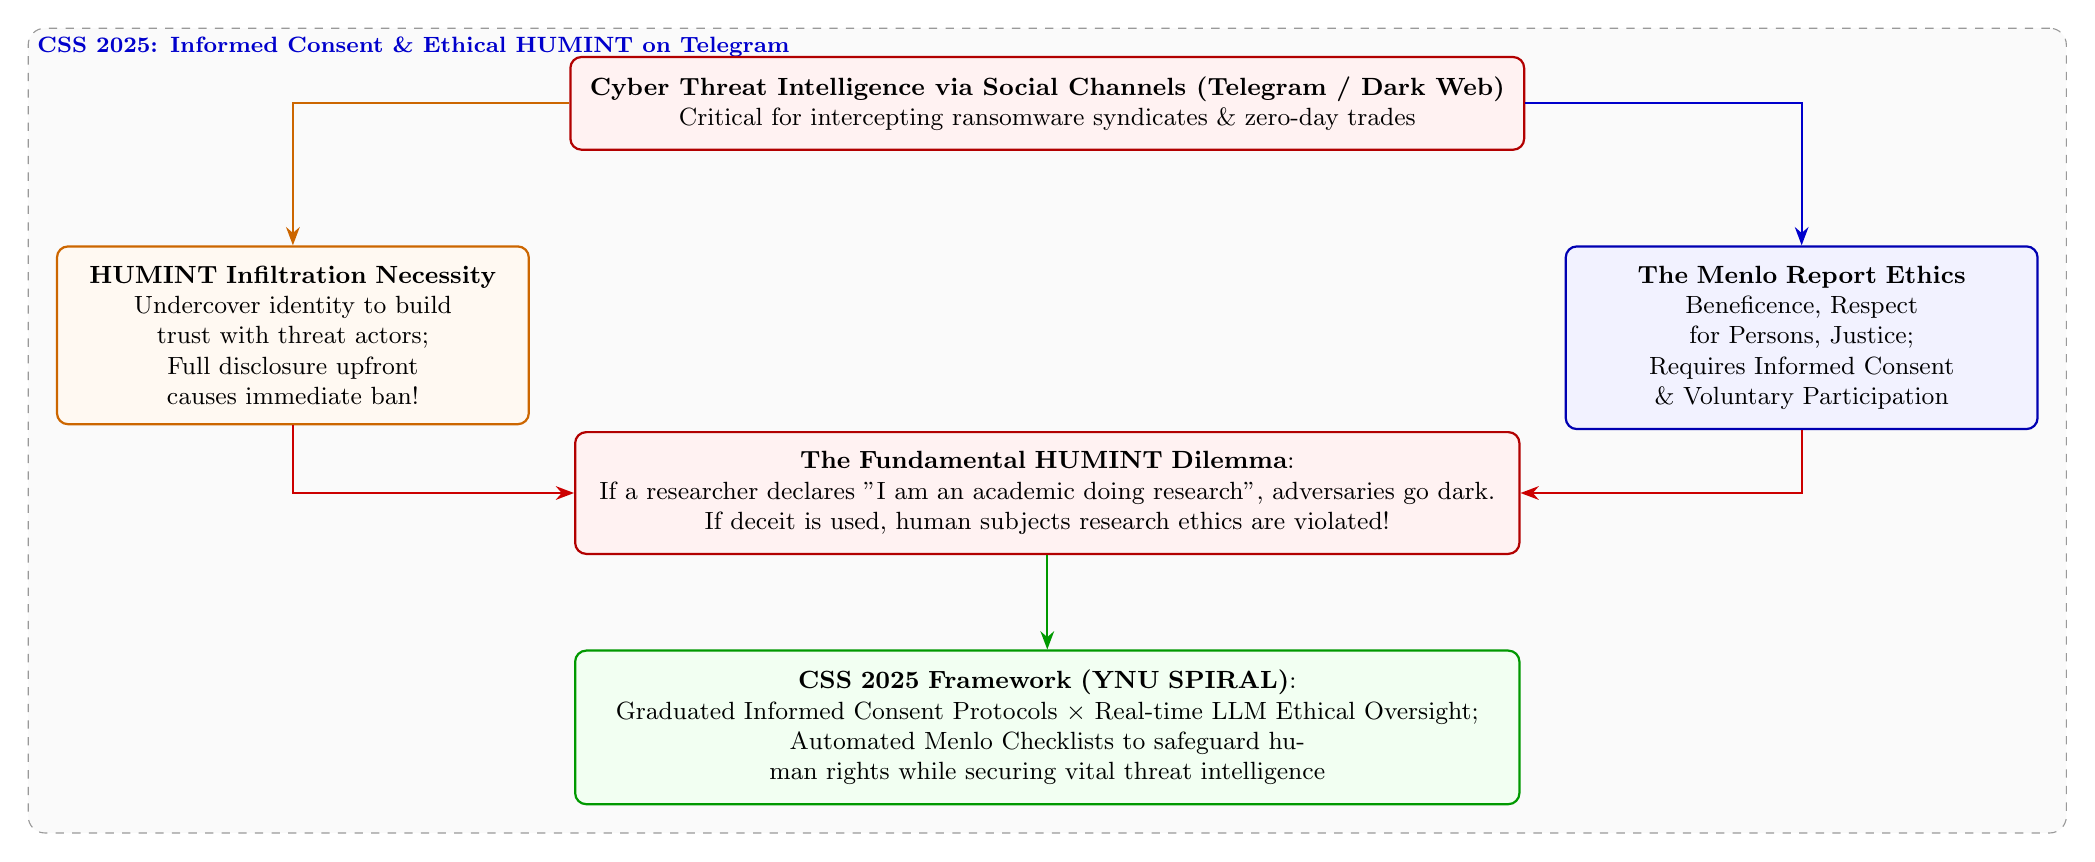
\begin{tikzpicture}[
    font=\small,
    >=Stealth,
    node distance=1.2cm,
    block/.style={rectangle, draw=blue!70!black, fill=blue!5, rounded corners=4pt, thick, align=center, inner sep=7pt},
    alertblock/.style={rectangle, draw=red!70!black, fill=red!5, rounded corners=4pt, thick, align=center, inner sep=7pt},
    greenblock/.style={rectangle, draw=green!60!black, fill=green!5, rounded corners=4pt, thick, align=center, inner sep=7pt},
    amberblock/.style={rectangle, draw=orange!80!black, fill=orange!5, rounded corners=4pt, thick, align=center, inner sep=7pt},
    groupbox/.style={draw=black!40, dashed, rounded corners=6pt, fill=black!2, inner sep=10pt}
]

    % Top Problem
    \node[alertblock] (threat) {\textbf{Cyber Threat Intelligence via Social Channels (Telegram / Dark Web)}\\Critical for intercepting ransomware syndicates \& zero-day trades};

    % Two Pillars: Operational Feasibility vs Ethical Principles
    \node[amberblock, below left=1.2cm and 0.5cm of threat, text width=5.5cm] (humanint) {\textbf{HUMINT Infiltration Necessity}\\Undercover identity to build trust with threat actors;\\Full disclosure upfront causes immediate ban!};

    \node[block, below right=1.2cm and 0.5cm of threat, text width=5.5cm] (menlo) {\textbf{The Menlo Report Ethics}\\Beneficence, Respect for Persons, Justice;\\Requires Informed Consent \& Voluntary Participation};

    \draw[->, thick, orange!80!black] (threat) -| (humanint);
    \draw[->, thick, blue!80!black] (threat) -| (menlo);

    % Central Conflict & Dilemma
    \node[alertblock, below=1.2cm of $(humanint)!0.5!(menlo)$, text width=11.5cm] (dilemma) {\textbf{The Fundamental HUMINT Dilemma}:\\If a researcher declares "I am an academic doing research", adversaries go dark.\\If deceit is used, human subjects research ethics are violated!};

    \draw[->, thick, red!80!black] (humanint) |- (dilemma);
    \draw[->, thick, red!80!black] (menlo) |- (dilemma);

    % Solution: YNU SPIRAL Framework
    \node[greenblock, below=1.2cm of dilemma, text width=11.5cm] (solution) {\textbf{CSS 2025 Framework (YNU SPIRAL)}:\\Graduated Informed Consent Protocols $\times$ Real-time LLM Ethical Oversight;\\Automated Menlo Checklists to safeguard human rights while securing vital threat intelligence};

    \draw[->, thick, green!60!black] (dilemma) -- (solution);

    \begin{scope}[on background layer]
        \node[groupbox, fit=(threat) (humanint) (menlo) (dilemma) (solution), label={[anchor=north west, font=\footnotesize\bfseries, blue!80!black]north west:CSS 2025: Informed Consent \& Ethical HUMINT on Telegram}] {};
    \end{scope}

\end{tikzpicture}
\end{document}
